\subsection{Digital Compass Operation}
A digital compass was implemented into the system to account for the sensor suite's rotation.This was accomplished through the use of a magnetometer. A magnetometer is a digital instrument that measures the direction of a magnetic field at a point in space. Magnetometers are commonly found in Inertial Measurement Units (IMUs).

\subsubsection{Selection}
This project required a sensitive IMU that was able to provide accurate and repeatable compass directions. Due to the time limitations and budgetary restrictions of this project, the PmodNAV IMU was selected. The PmodNAV provided 10-degree of freedom functionality through its on-chip LSM9DS1 3-axis magnetometer, 3-axis accelerometer, and 3-axis gyroscope, and the LPS25HB barometer \cite{lsm9ds1, lps25hd}. The PmodNAV is shown in Figure \ref{pmodnav}.

\begin{figure}[H]
	\centerline{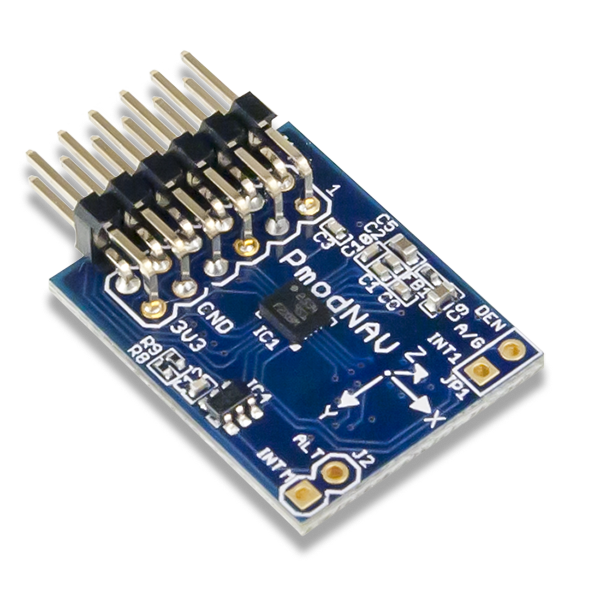
\includegraphics[width=0.5\textwidth]{pmodnav.png}}
	\caption{The PmodNAV 10-Axis IMU \cite{pmodnav_ref}}
	\label{pmodnav}
\end{figure}

The PmodNAV's was easy to integrate into this design, as it was fixed in position connected to the ZedBoard and its communication was directly compatible, requiring no intermediary hardware.

\subsubsection{Communication}
The PmodNAV supported two communication protocols: Serial Peripheral Interface (SPI) and Inter-Integrated Circuit (I\textsuperscript{2}C) \cite{lsm9ds1}. However the magnetometer on the LSM9DS1 was not addressable by the I\textsuperscript{2}C bus, so SPI communication was implemented. The magnetometer's SPI protocol is shown in Figure \ref{magnetometer_spi}.

\begin{figure}[H]
	\centerline{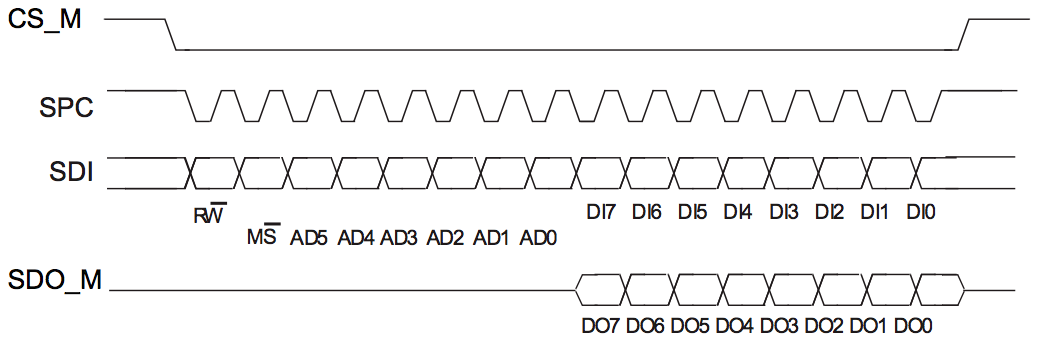
\includegraphics[width=1\textwidth]{magnetometer_spi.png}}
	\caption{Magnetometer SPI Read and Write Protocol \cite{lsm9ds1}}
	\label{magnetometer_spi}
\end{figure}

The CS\textunderscore{}M line was the magnetometer active-low chip select. The SPC line is the clock controlled by the master. SDI and SDO\textunderscore{}M are the data input and data output lines, respectively. They were driven at the falling edge of SPC and were captured at the rising edge \cite{lsm9ds1}.
\par
In an SPI sequence, the first bit sent from the master is the read/write bit, $R\overline{W}$. This bit was set to 1 to read from the compass, and 0 for a write to the compass. For a read sequence, the $DO$ bits represented the data read from the memory address specified by the $AD$ bits. The $DI$ bits were not written to. For a write sequence, the $DI$ bits were the data being written to the memory address, and the $DO$ line was ignored. When the $M\overline{S}$ bit was set to 1 the memory address signified by the address bits $AD5$ down to $AD0$ was auto-incremented, allowing for multiple reads or writes to be completed in the same SPI transaction \cite{lsm9ds1}. Figure \ref{multiple_reads} shows a multiple-byte SPI read protocol. 

\begin{figure}[H]
	\centerline{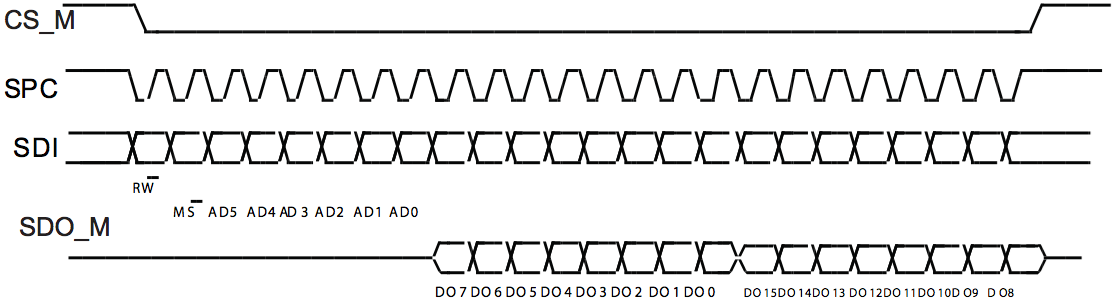
\includegraphics[width=1\textwidth]{multiple_reads.png}}
	\caption{Magnetometer Multiple-Byte SPI Read Protocol \cite{lsm9ds1}}
	\label{multiple_reads}
\end{figure}

\subsubsection{Register Settings} \label{imu_settings}
The magnetometer on the LSM9DS1 needed slight adjustments in its register setting in order to operate properly. The adjustments were done by writing to the magnetometer's control registers.
\par
One register that was written to was the magnetometer's control register 1, CTRL\textunderscore{}REG\textunderscore{}1\textunderscore{}M, at address 20\textsubscript{16}. 7C\textsubscript{16} was written to CTRL\textunderscore{}REG\textunderscore{}1\textunderscore{}M to signify ultra high performance mode for the magnetometer's x- and y-axis \cite{lsm9ds1}.
\par
The other register that was written to was the magnetometer's control register 3, CTRL\textunderscore{}REG\textunderscore{}3\textunderscore{}M, at address 22\textsubscript{16}. 80\textsubscript{16} was written to CTRL\textunderscore{}REG\textunderscore{}3\textunderscore{}M to turn off I\textsuperscript{2}C and turn on the magnetometer in the continuous-conversion mode \cite{lsm9ds1}.
\par
Due to time constraints, the magnetometer on the PmodNAV was the only slave that was interfaced to. The accelerometer, gyroscope, and barometer were not used so the above control registers did not need to be changed to allow the other sensors to be read from.

\subsubsection{Read Registers}
With the magnetometer turned on and its settings properly adjusted, its data registers were read from. As such, the $R\overline{W}$ bit was set to 1. There were two different read sequences used to obtain compass data. 
\par
One sequence that was used was a read from the status register, STATUS\textunderscore{}REG\textunderscore{}M, which is at address 27\textsubscript{16}. The status register signifies which of the magnetometer's registers hold data that has not yet been read. This address was read from until the two least significant data bits read 11\textsubscript{2}, signifying that new x- and y-axis magnetometer data was available \cite{lsm9ds1}. Once new x- and y-axis data was available, the corresponding data registers were read from.
\par
The next command was used to read the available x- and y-axis magnetometer data. This data came in 16-bit resolution. Due to the SPI transfer protocol shown in Figure \ref{magnetometer_spi}, data was read 8 bits at a time MSB first. Since each axis had 16-bit resolution, each axis had two addresses containing 8-bit data words. The x- and y-data addresses were consecutive, allowing 32 bits of data to be obtained in one cascading read in the format shown in Figure \ref{multiple_reads}. The cascading read was performed from address 28\textsubscript{16}, OUT\textunderscore{}X\textunderscore{}L\textunderscore{}M, to obtain the x-axis lower word, the x-axis upper word, the y-axis lower word, and then the y-axis upper word \cite{lsm9ds1}.







